\documentclass[11pt]{article}
\usepackage{outlines}
\usepackage{graphicx}
\usepackage[T1]{fontenc}
\usepackage{subcaption}
\usepackage[margin=1in]{geometry}

\usepackage{geometry}
\usepackage[square,sort,comma,numbers,super]{natbib}
\usepackage{pdflscape}
\usepackage[colorlinks,allcolors=blue]{hyperref}
\usepackage{afterpage}

\usepackage[utf8]{inputenc}
\usepackage{xcolor}
\definecolor{textblue}{rgb}{.2,.2,.7}
\definecolor{textred}{rgb}{0.54,0,0}
\definecolor{textgreen}{rgb}{0,0.43,0}

\usepackage{enumitem}
\setlist{nosep}

\usepackage{listings}
\usepackage[export]{adjustbox}
\usepackage{wrapfig}



\lstset{language=Java, 
lineskip=-.1cm,
stepnumber=1,
numbersep=2pt, 
tabsize=4,
basicstyle=\ttfamily,
keywordstyle=\color{textblue},
commentstyle=\color{textred},   
stringstyle=\color{textgreen},
frame=none,                    
columns=fullflexible,
keepspaces=true,
xleftmargin=\parindent,
showstringspaces=false}

\graphicspath{ {./images/} }

\setlength{\parindent}{0pt}

% pt = project title; shorthand
\newcommand{\pt}{Multi-User Poker Game}
\newcommand{\pn}{Rekop}

\title{Dissertation \pt}
\author{James Scully}

\setcounter{tocdepth}{4}
\setcounter{secnumdepth}{5}



\begin{document}

{\fontfamily{cmss}\selectfont}



\newcommand{\cardheight}{6em}

\newcommand{\tenclubs}{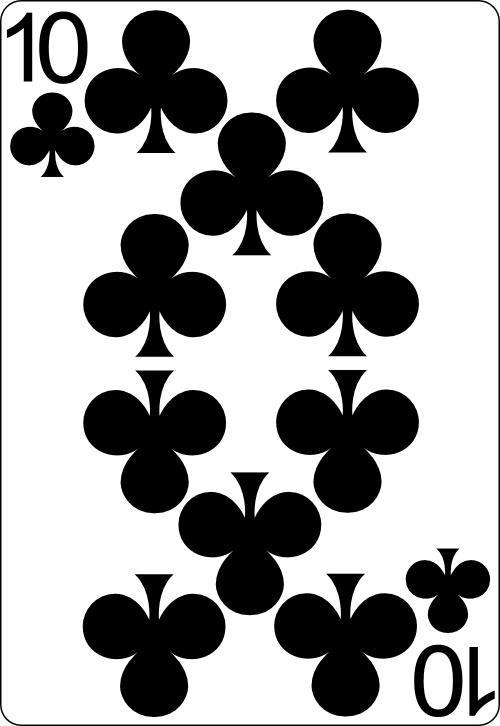
\includegraphics[height=\cardheight]{cards/10_of_clubs.png}}
\newcommand{\tendiamonds}{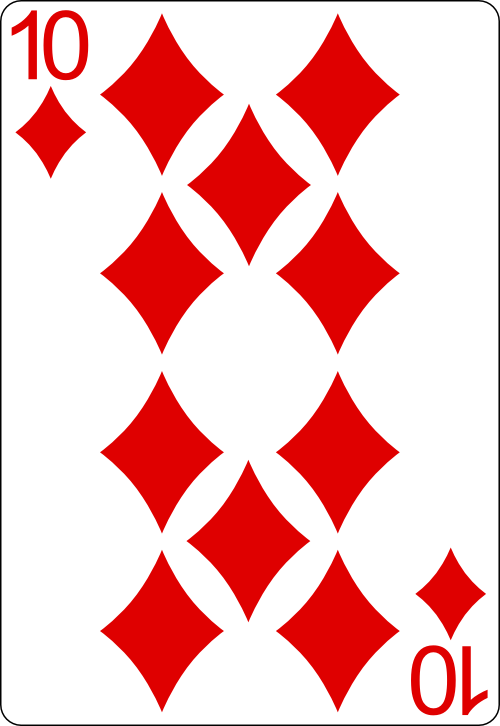
\includegraphics[height=\cardheight]{cards/10_of_diamonds.png}}
\newcommand{\tenhearts}{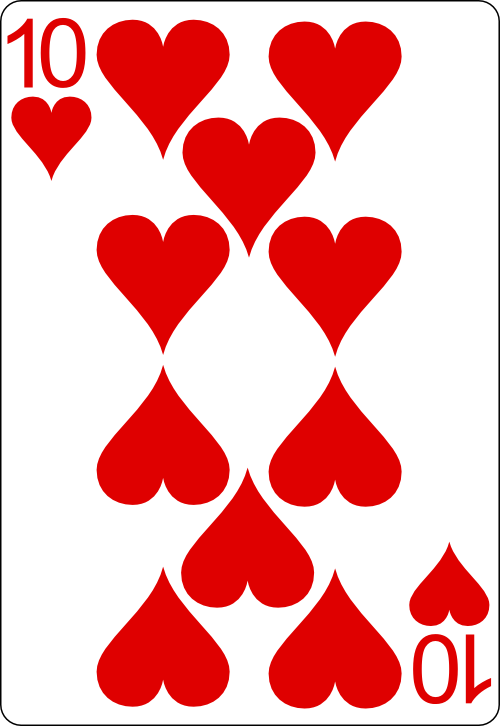
\includegraphics[height=\cardheight]{cards/10_of_hearts.png}}
\newcommand{\tenspades}{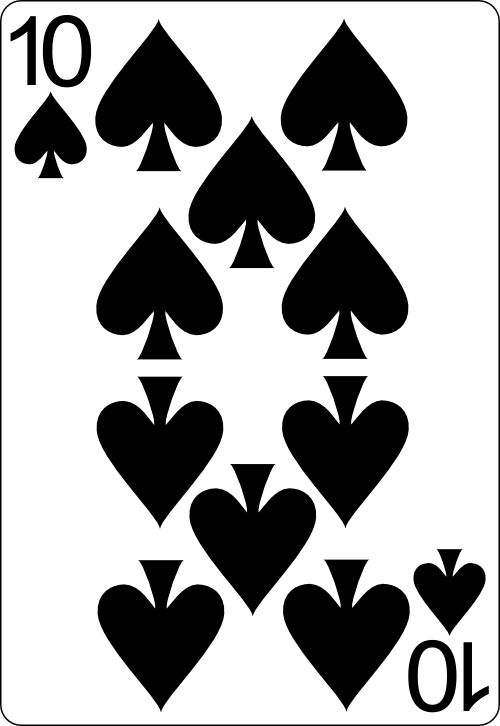
\includegraphics[height=\cardheight]{cards/10_of_spades.png}}
\newcommand{\twoclubs}{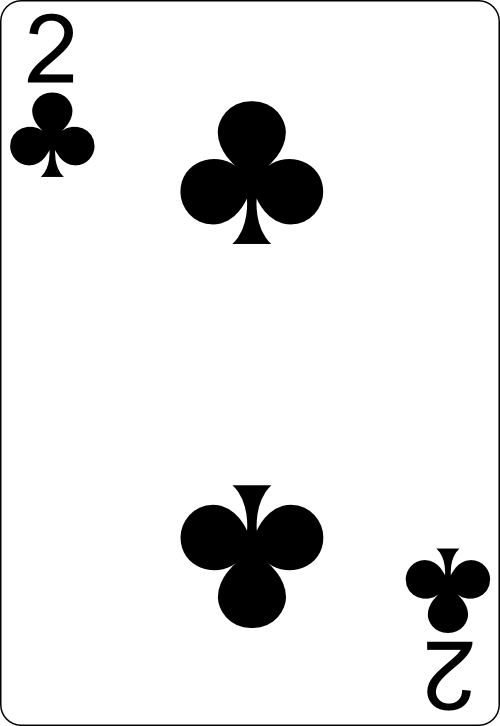
\includegraphics[height=\cardheight]{cards/2_of_clubs.png}}
\newcommand{\twodiamonds}{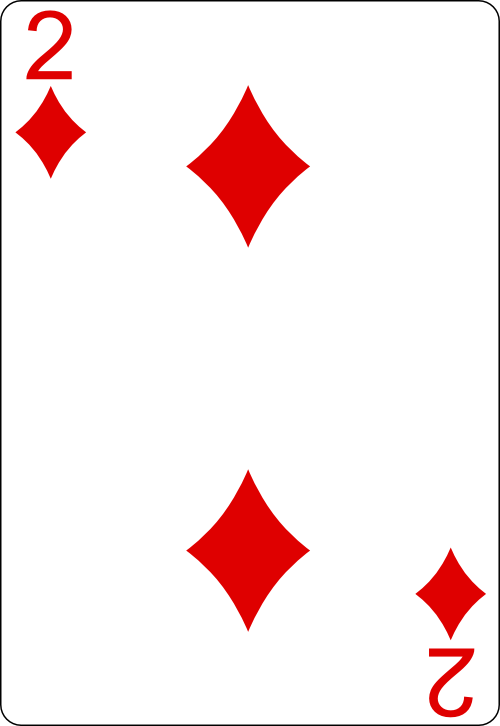
\includegraphics[height=\cardheight]{cards/2_of_diamonds.png}}
\newcommand{\twohearts}{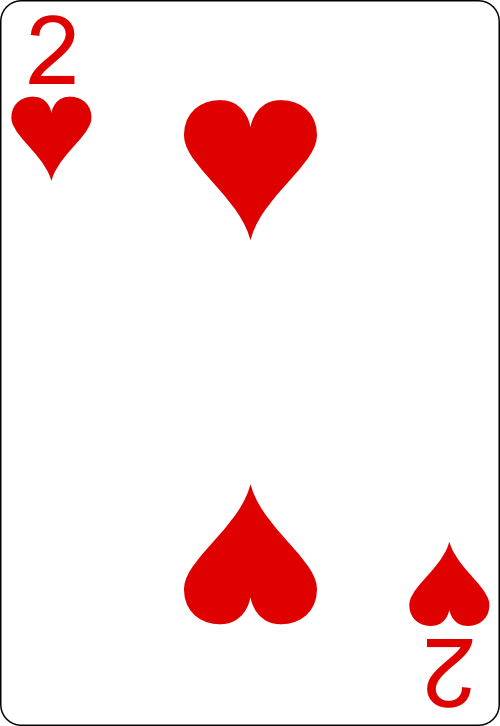
\includegraphics[height=\cardheight]{cards/2_of_hearts.png}}
\newcommand{\twospades}{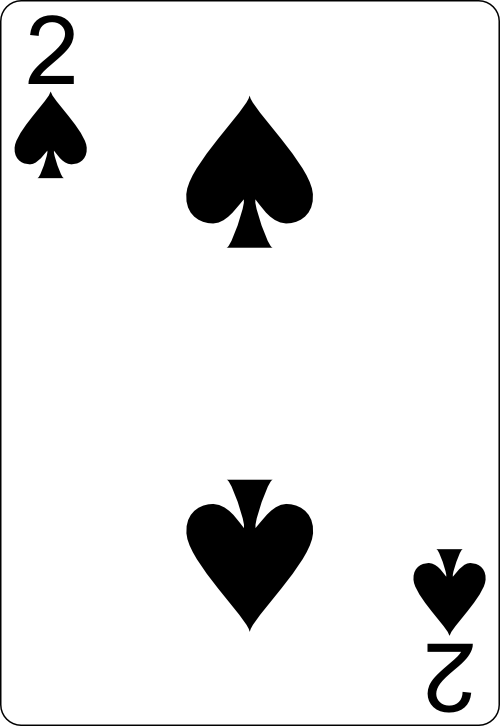
\includegraphics[height=\cardheight]{cards/2_of_spades.png}}
\newcommand{\threeclubs}{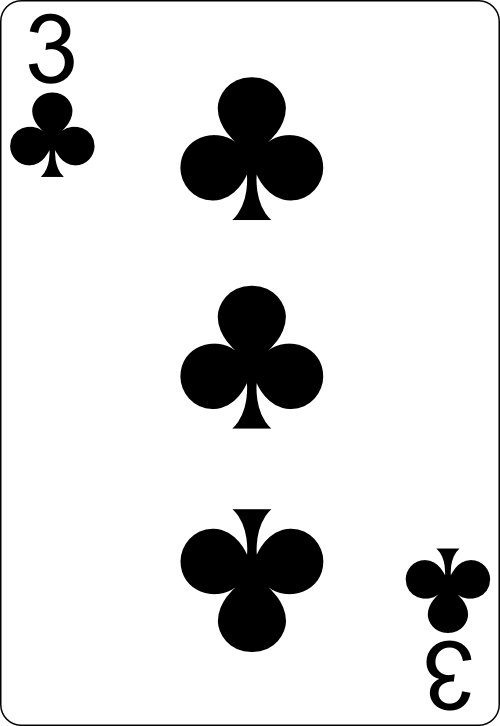
\includegraphics[height=\cardheight]{cards/3_of_clubs.png}}
\newcommand{\threediamonds}{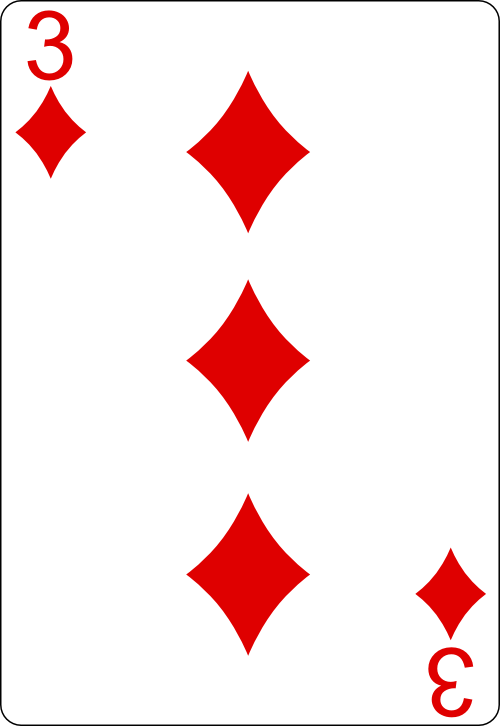
\includegraphics[height=\cardheight]{cards/3_of_diamonds.png}}
\newcommand{\threehearts}{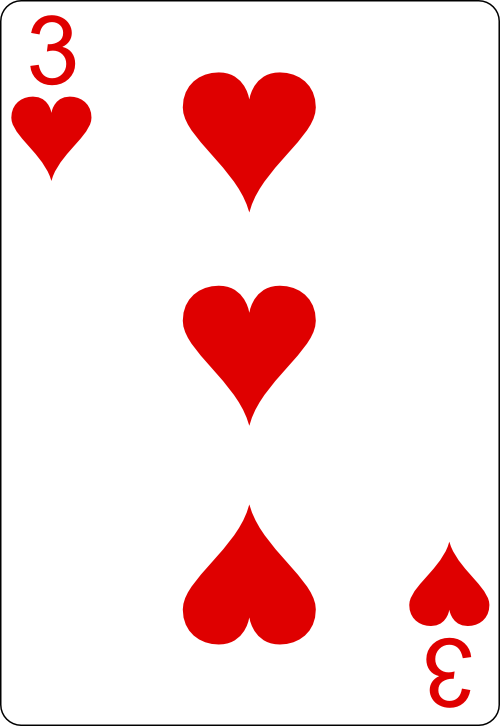
\includegraphics[height=\cardheight]{cards/3_of_hearts.png}}
\newcommand{\threespades}{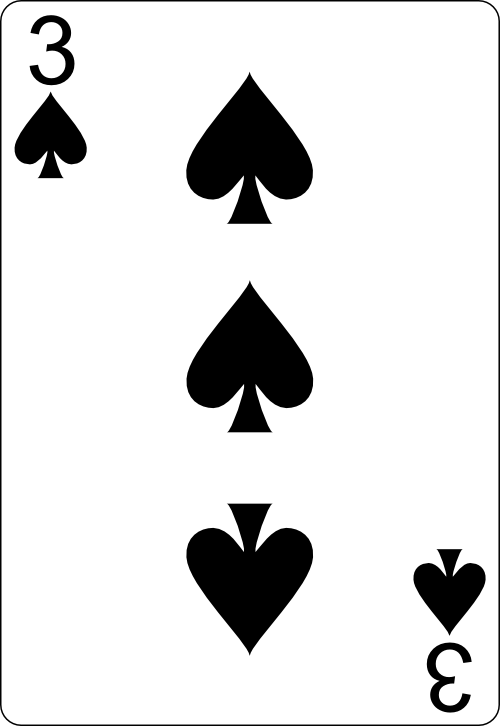
\includegraphics[height=\cardheight]{cards/3_of_spades.png}}
\newcommand{\fourclubs}{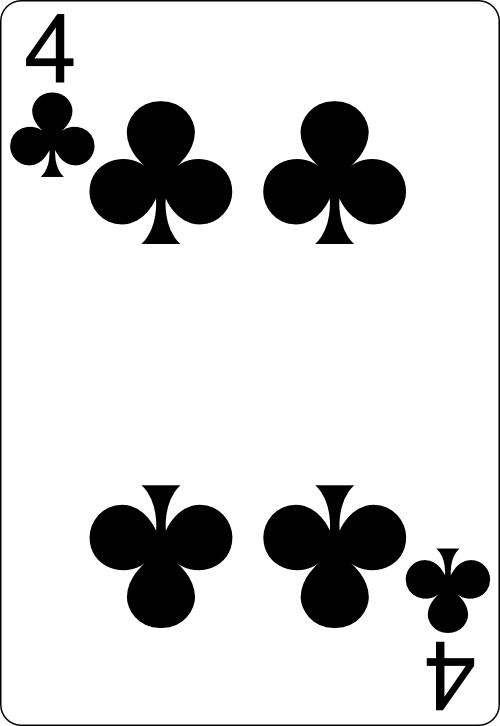
\includegraphics[height=\cardheight]{cards/4_of_clubs.png}}
\newcommand{\fourdiamonds}{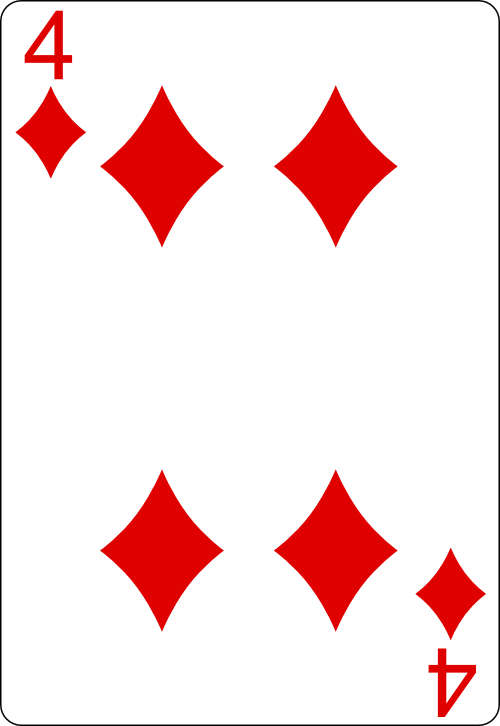
\includegraphics[height=\cardheight]{cards/4_of_diamonds.png}}
\newcommand{\fourhearts}{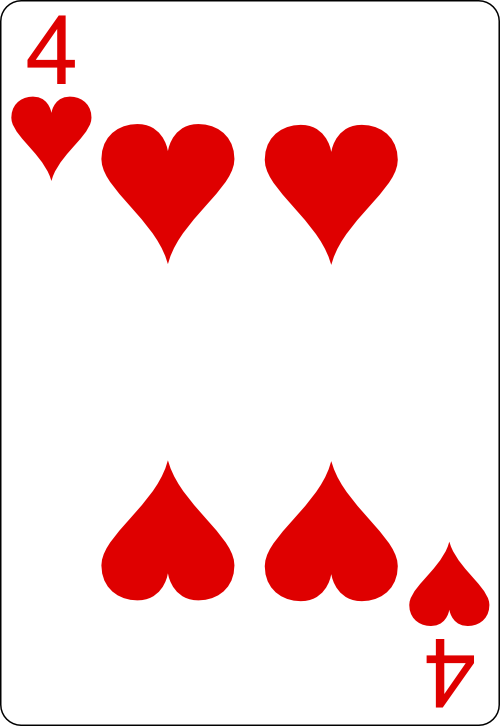
\includegraphics[height=\cardheight]{cards/4_of_hearts.png}}
\newcommand{\fourspades}{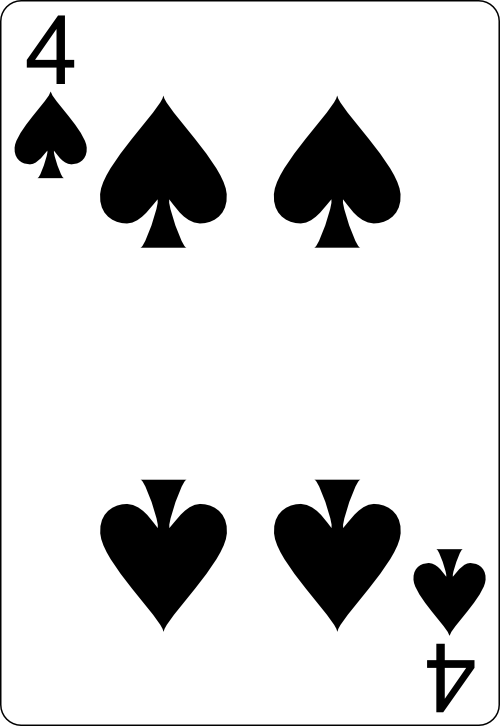
\includegraphics[height=\cardheight]{cards/4_of_spades.png}}
\newcommand{\fiveclubs}{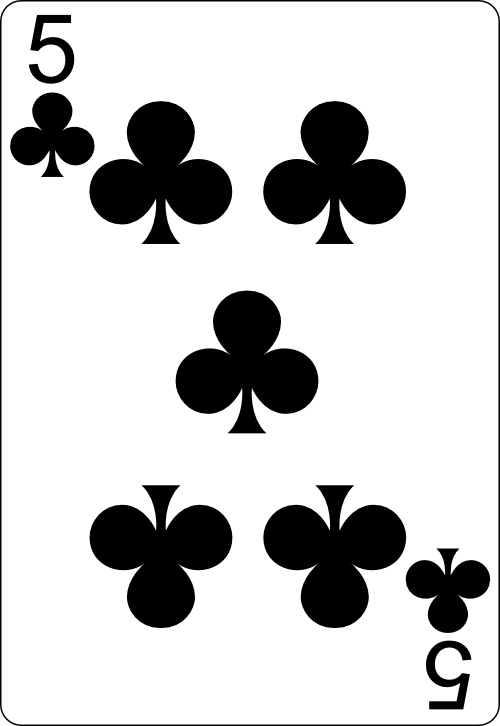
\includegraphics[height=\cardheight]{cards/5_of_clubs.png}}
\newcommand{\fivediamonds}{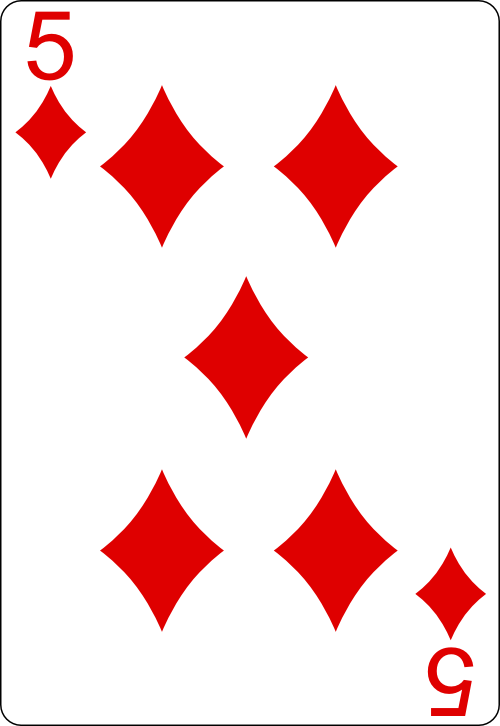
\includegraphics[height=\cardheight]{cards/5_of_diamonds.png}}
\newcommand{\fivehearts}{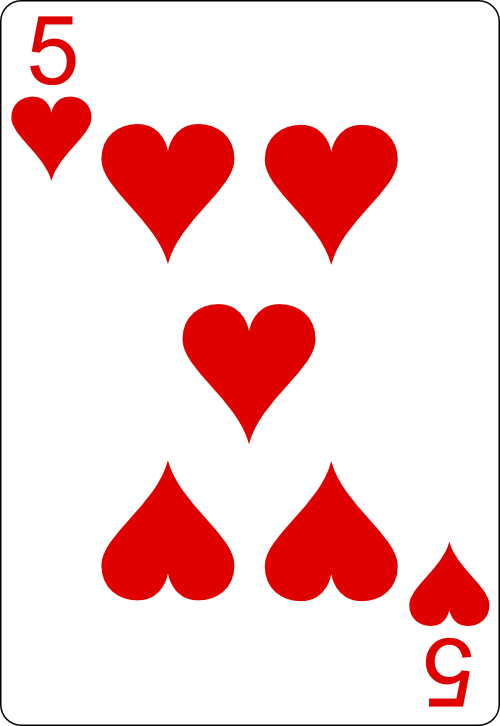
\includegraphics[height=\cardheight]{cards/5_of_hearts.png}}
\newcommand{\fivespades}{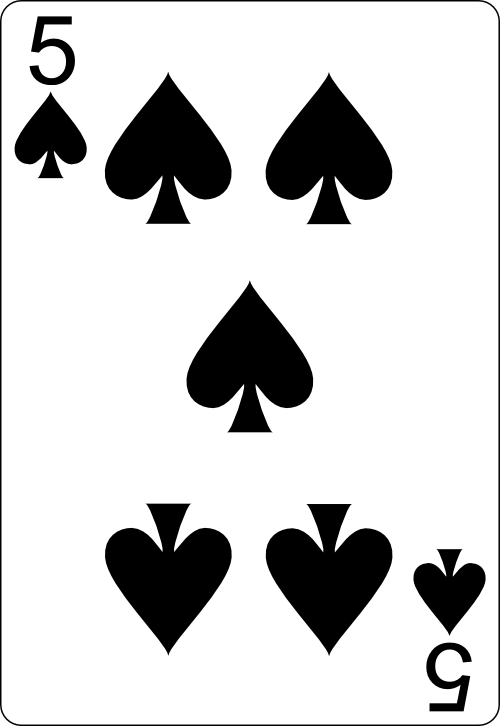
\includegraphics[height=\cardheight]{cards/5_of_spades.png}}
\newcommand{\sixclubs}{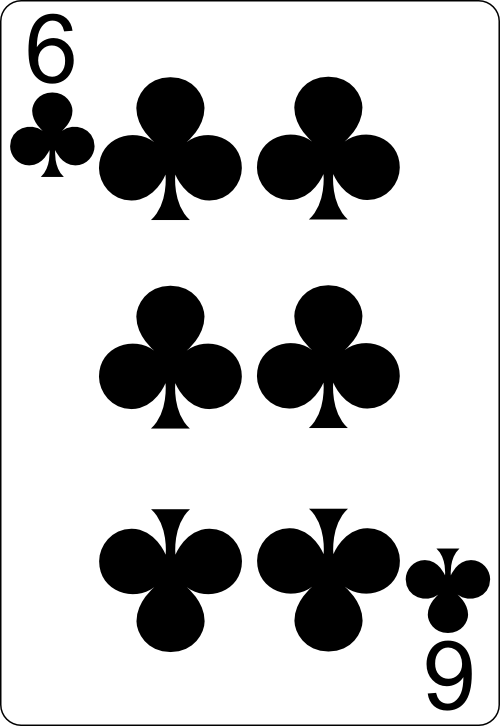
\includegraphics[height=\cardheight]{cards/6_of_clubs.png}}
\newcommand{\sixdiamonds}{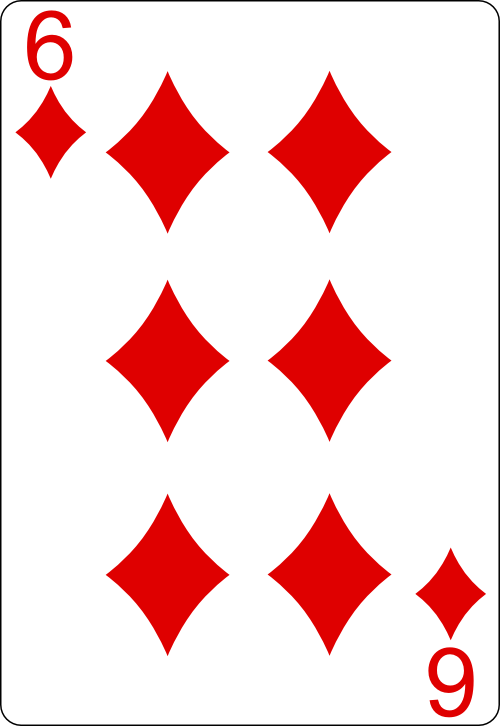
\includegraphics[height=\cardheight]{cards/6_of_diamonds.png}}
\newcommand{\sixhearts}{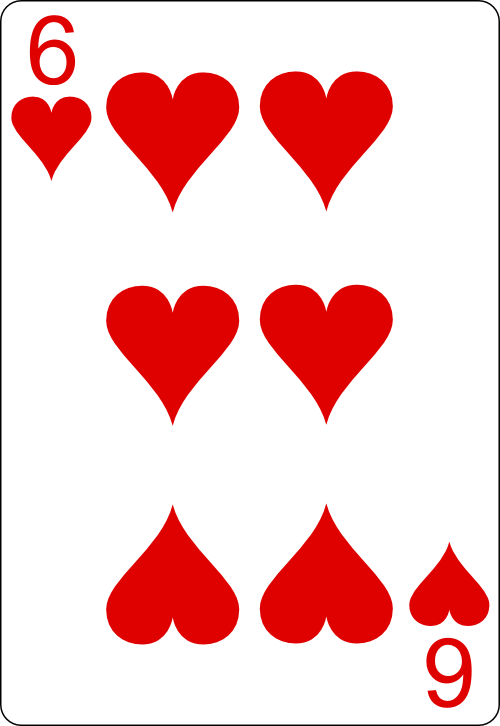
\includegraphics[height=\cardheight]{cards/6_of_hearts.png}}
\newcommand{\sixspades}{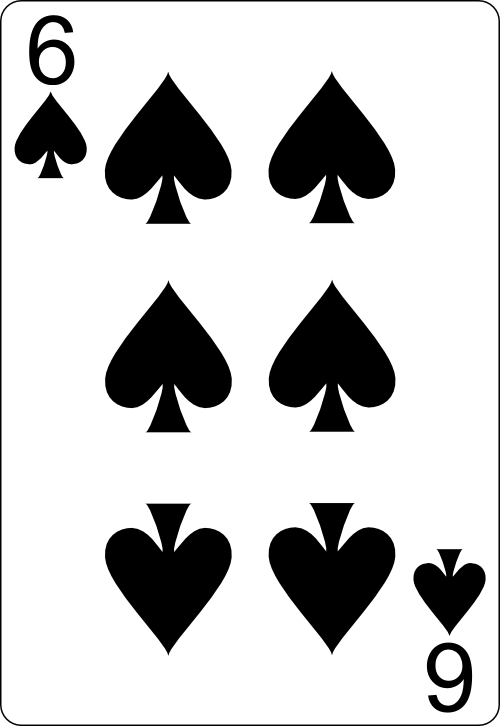
\includegraphics[height=\cardheight]{cards/6_of_spades.png}}
\newcommand{\sevenclubs}{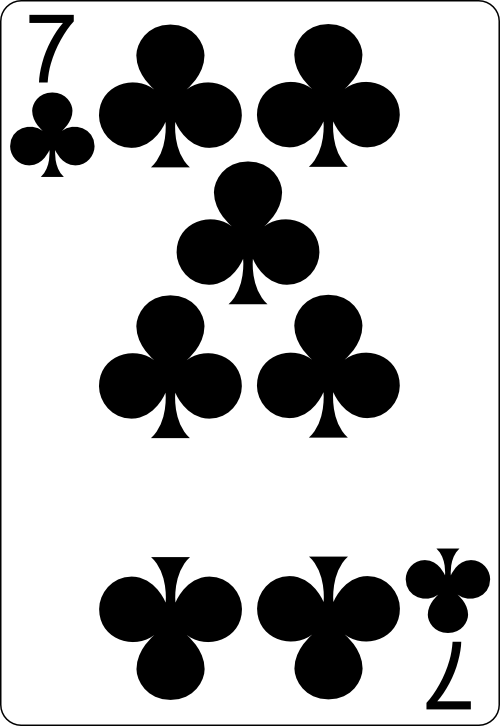
\includegraphics[height=\cardheight]{cards/7_of_clubs.png}}
\newcommand{\sevendiamonds}{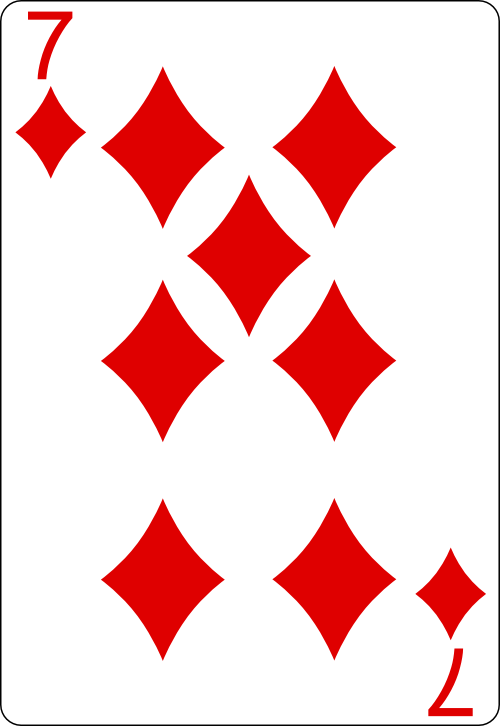
\includegraphics[height=\cardheight]{cards/7_of_diamonds.png}}
\newcommand{\sevenhearts}{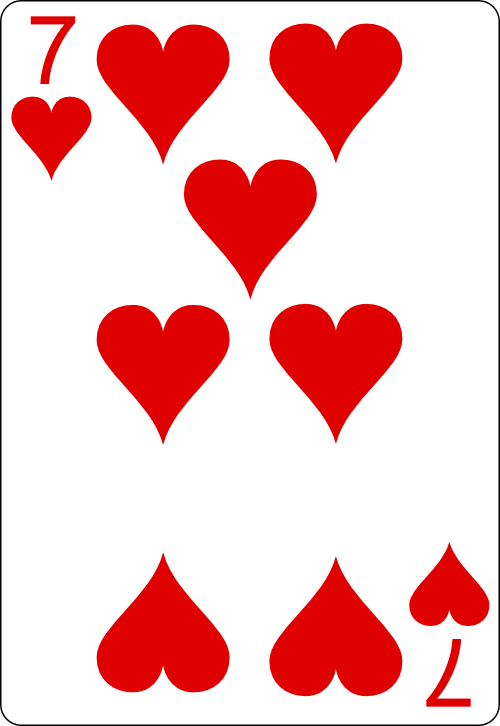
\includegraphics[height=\cardheight]{cards/7_of_hearts.png}}
\newcommand{\sevenspades}{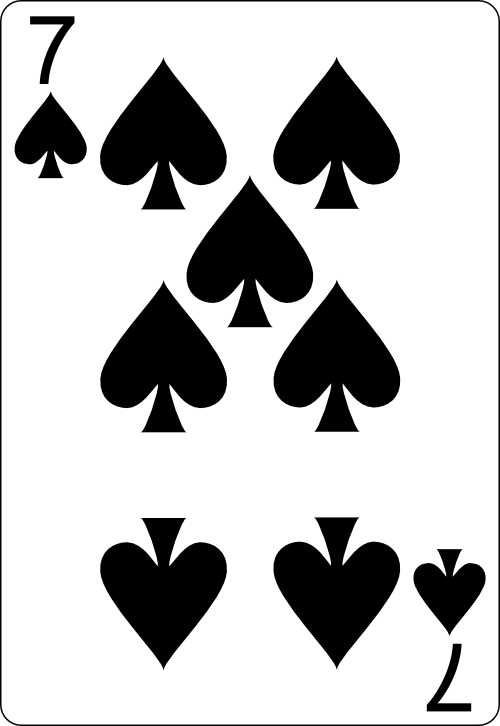
\includegraphics[height=\cardheight]{cards/7_of_spades.png}}
\newcommand{\eightclubs}{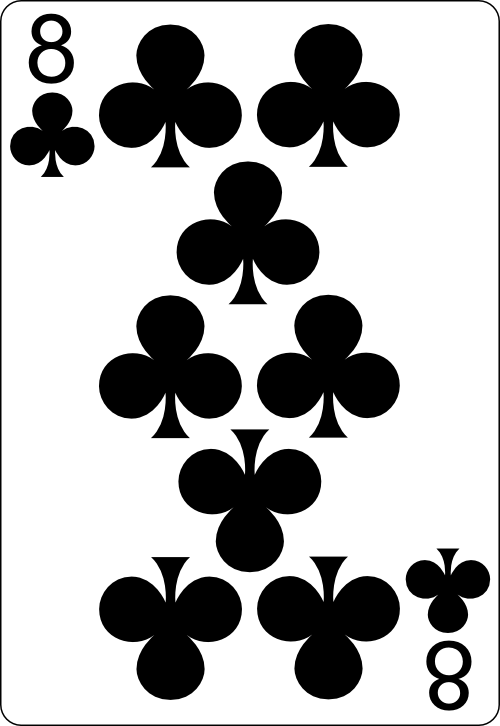
\includegraphics[height=\cardheight]{cards/8_of_clubs.png}}
\newcommand{\eightdiamonds}{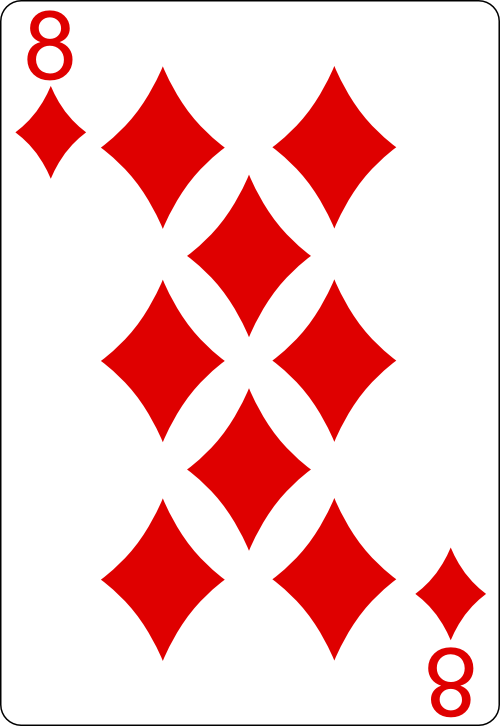
\includegraphics[height=\cardheight]{cards/8_of_diamonds.png}}
\newcommand{\eighthearts}{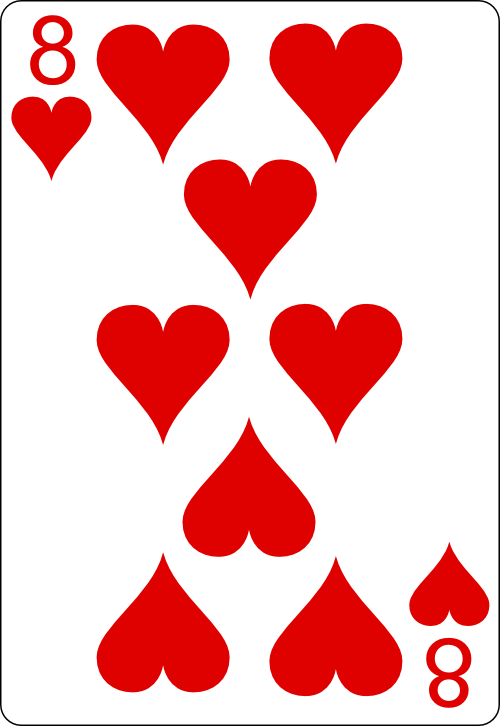
\includegraphics[height=\cardheight]{cards/8_of_hearts.png}}
\newcommand{\eightspades}{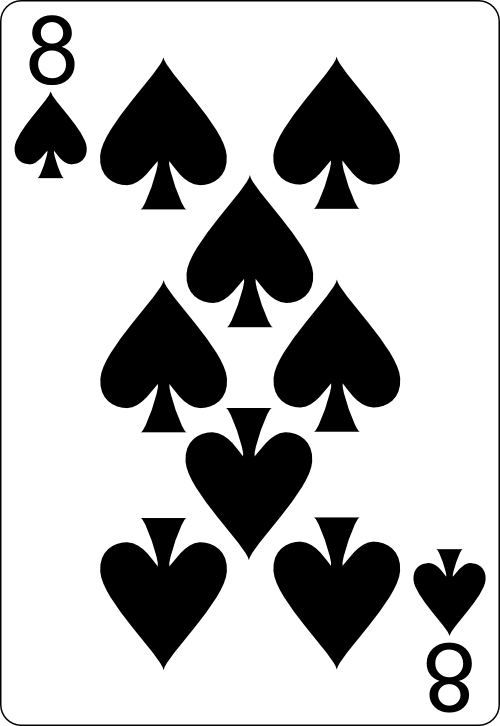
\includegraphics[height=\cardheight]{cards/8_of_spades.png}}
\newcommand{\nineclubs}{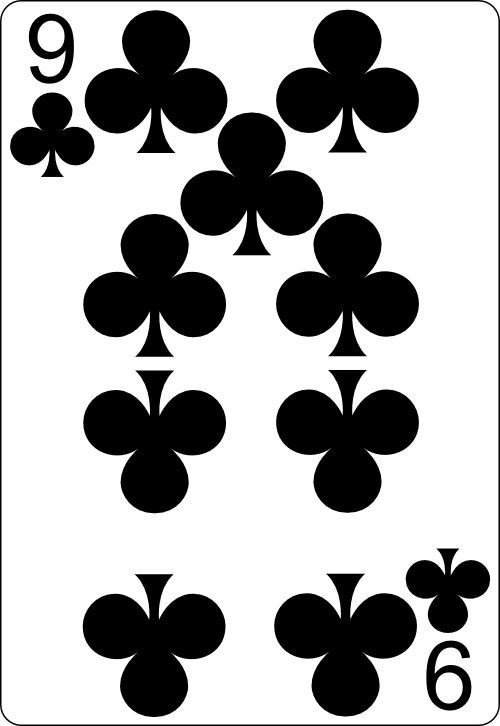
\includegraphics[height=\cardheight]{cards/9_of_clubs.png}}
\newcommand{\ninediamonds}{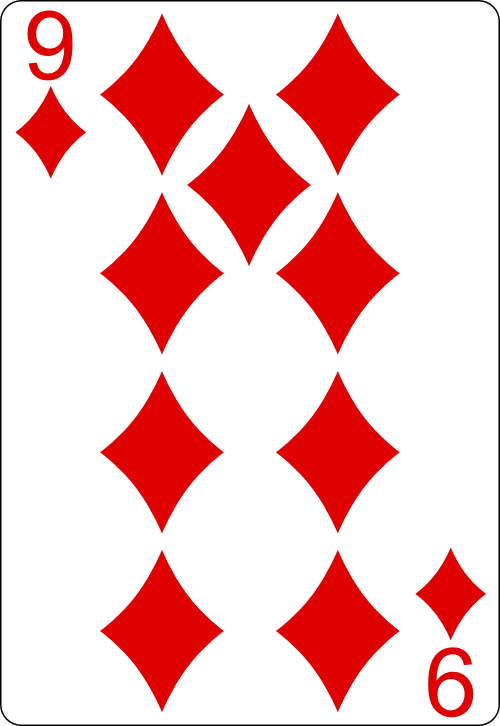
\includegraphics[height=\cardheight]{cards/9_of_diamonds.png}}
\newcommand{\ninehearts}{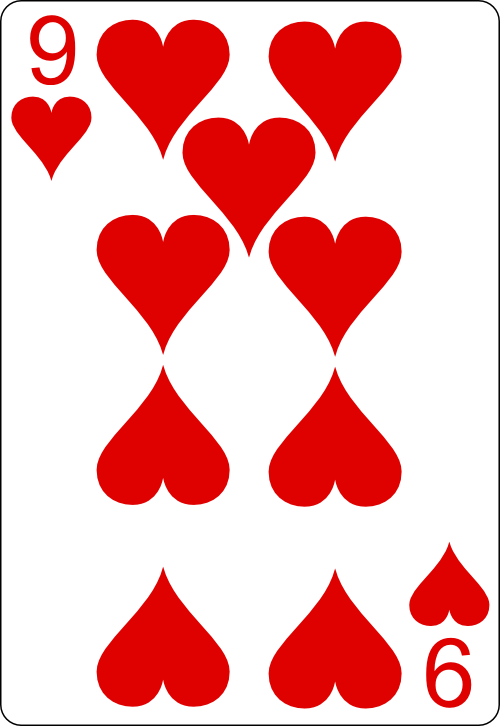
\includegraphics[height=\cardheight]{cards/9_of_hearts.png}}
\newcommand{\ninespades}{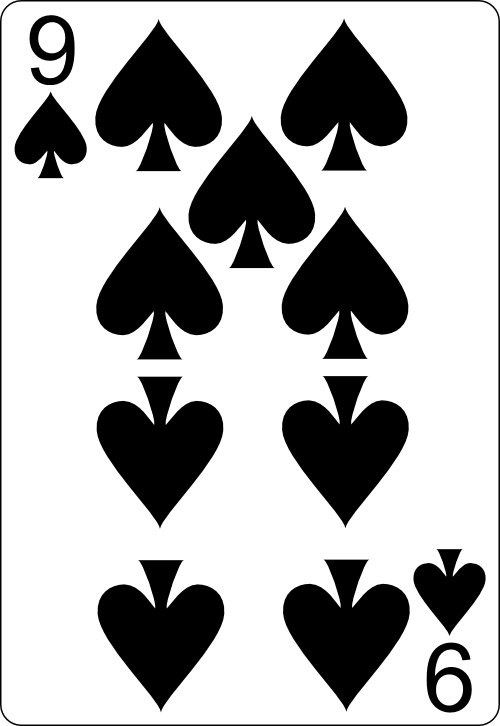
\includegraphics[height=\cardheight]{cards/9_of_spades.png}}
\newcommand{\aceclubs}{
\includegraphics[height=\cardheight]{cards/ace_of_clubs.png}}
\newcommand{\acediamonds}{
\includegraphics[height=\cardheight]{cards/ace_of_diamonds.png}}
\newcommand{\acehearts}{
\includegraphics[height=\cardheight]{cards/ace_of_hearts.png}}
\newcommand{\acespades}{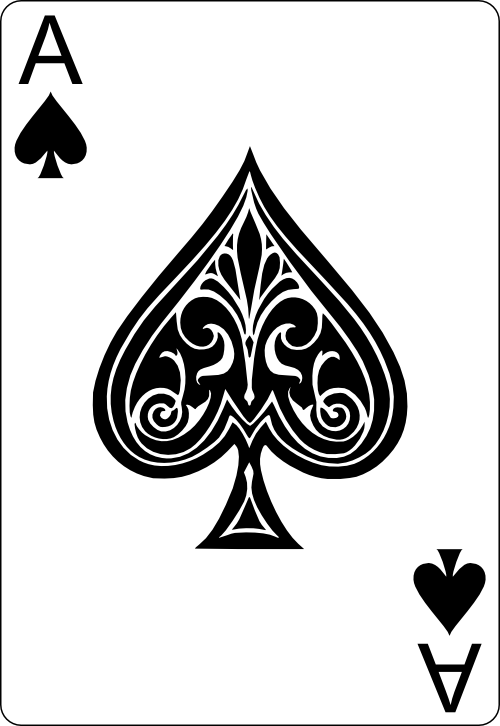
\includegraphics[height=\cardheight]{cards/ace_of_spades.png}}
\newcommand{\jackclubs}{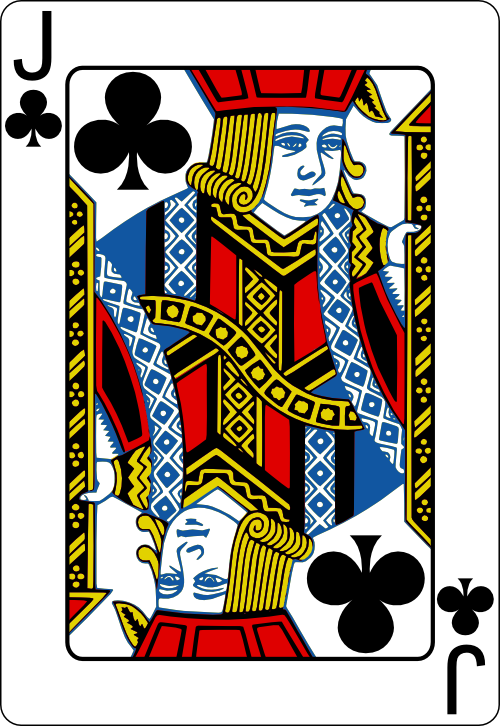
\includegraphics[height=\cardheight]{cards/jack_of_clubs.png}}
\newcommand{\jackdiamonds}{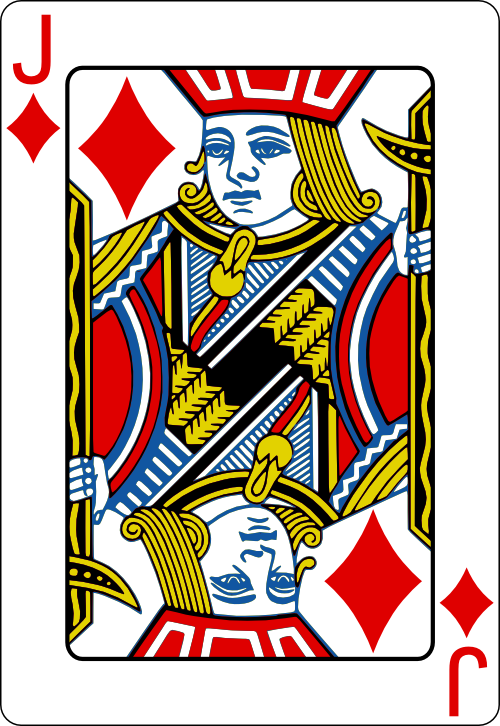
\includegraphics[height=\cardheight]{cards/jack_of_diamonds.png}}
\newcommand{\jackhearts}{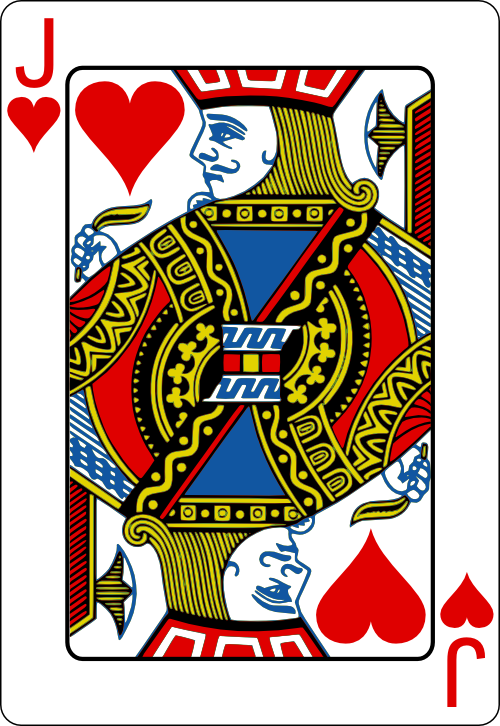
\includegraphics[height=\cardheight]{cards/jack_of_hearts.png}}
\newcommand{\jackspades}{
\includegraphics[height=\cardheight]{cards/jack_of_spades.png}}
\newcommand{\kingclubs}{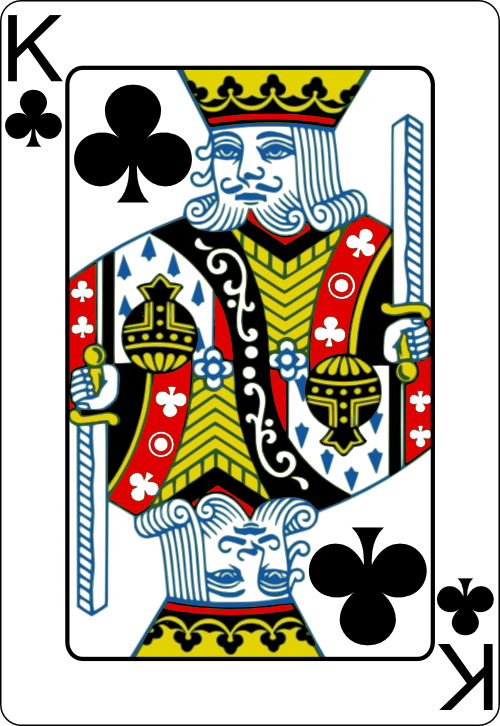
\includegraphics[height=\cardheight]{cards/king_of_clubs.png}}
\newcommand{\kingdiamonds}{
\includegraphics[height=\cardheight]{cards/king_of_diamonds.png}}
\newcommand{\kinghearts}{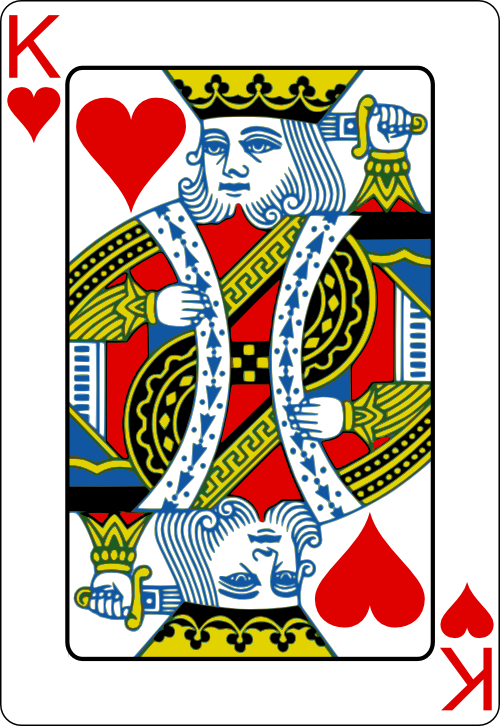
\includegraphics[height=\cardheight]{cards/king_of_hearts.png}}
\newcommand{\kingspades}{
\includegraphics[height=\cardheight]{cards/king_of_spades.png}}
\newcommand{\queenclubs}{
\includegraphics[height=\cardheight]{cards/queen_of_clubs.png}}
\newcommand{\queendiamonds}{
\includegraphics[height=\cardheight]{cards/queen_of_diamonds.png}}
\newcommand{\queenhearts}{\includegraphics[height=\cardheight]{cards/queen_of_hearts.png}}
\newcommand{\queenspades}{\includegraphics[height=\cardheight]{cards/queen_of_spades.png}}

\hspace{0pt}

\vfill

\begin{center}
	\includegraphics[scale=0.4]{uni_logo}
	
	\vspace{1cm}
	
	{\Large \textbf{Dissertation\\} 
		\vspace{16pt}
		Multi-User Interactive Delay-Tolerant Network\\
		\vspace{16pt}
		\textit{Rekop Poker}} 		
		\linebreak
		
	\textbf{I hereby declare that this dissertation is all my own work, \\except as indicated in the text} \\
	\vspace{8pt}
	\textbf{Signature}: J. W. Scully \\
	\textbf{Date}: 4/5/2020 \linebreak
		
	\begin{large}
		James Scully (14304469) \\
		psyjs20@nottingham.ac.uk \\
		G400 Computer Science \linebreak \\ 
	\end{large}
	
\end{center}

\vfill

\begin{center}
	\textbf{Project Supervisor:} Milena Radenkovic
\end{center}

\hspace{0pt}

\pagebreak


\newcommand{\entry}[1]{
	\textbf{#1} - 
}

\newcommand{\TODO}[1]{
	\textbf{{\Large \emph{#1}}}
}



\tableofcontents



\newpage


%%%
% Page 1: 
%%%

\section{Introduction}

Poker is a type of card game that is played and watched in tournaments by many around the world. Because of it's wide popularity, it has spawned multiple types, the most popular one being Texas Hold'em, which is the main type used in both research \hyperlink{research_texas}{(A Gilpin, 2006)} and is the main variant used in the World Series of Poker \hyperlink{wsop_texas}{(WSOP, 2019)}. Other types include the similar yet lesser-known Omaha hold'em and Five-card draw; a simpler type of poker, which does not utilize the typical table seen in both hold'ems. \\

A common problem encountered with most networks is that the client or user of a service can have a weak or 'spotty' internet connection, whereby they may lose connectivity occasionally or in certain bursts. This is especially prevalent with mobile connections, where rural or otherwise distanced areas can have trouble holding a steady connection. In these cases, it is vital that both the client is able to use the network or join as normal and that the server does not grind to a halt waiting on this person or break due to it, known as a \textit{delay-tolerant network} (DTN).

Delay-tolerant networks have been especially important in the modern world since the advent of mobile devices and their surge in popularity. This is due to the fact that they do not have a regular stable internet connection like most desktop computers do and have the problem of losing signal due to physical movement or placement of the device. If a network cannot handle delay or dropouts from a mobile client gracefully this can have devastating impacts on data integrity or the overall function of the service. \\

Though the term mobile devices can insinuate the idea of mobile phones, mobile devices can range from not only a handheld phone but to vehicles, robotics, aeroplanes and satellites. Whilst data integrity to a mobile phone may not be incredibly important, data integrity is certainly incredibly important to an aeroplane or satellite, where a small error or wrong instruction can result in major failure. \\

The service must be able to realise that a device is either experiencing delay/dropouts and must respond accordingly; either by aiming to keep future data consistent with the previously sent data, or by accounting for the delay. \\


%When one looks for a casual poker game that offers power to the actual end user, rather than attempting to fish money it can be quite difficult to find. From the authors own personal experience and observations with free and open software, it can be quite difficult to implement in some areas (such as games), however the ability to control a game how you would like and the ability to not have to rely on companies servers, trudge through in-application payments and ads is a unseen experience today. Some also do not allow for players with unreliable connections to continue; they are simply dropped from the game.  \\

%I believe that many of these are far too focused on the financial aspect of the game and neglect the small groups whom simply would like another medium to play poker. This is because lobbies are often not customizable and will drop players whom do not have a good enough network connection to the lobby, so that more players are able to join.  \\

%To remedy these issues, Rekop poker will be developed to handle disconnections or unstable connections by reserving their place in the lobby and the ability to join back when the player is available to. It will also not feature micro-transactions and provide the ability for players to host their own servers, with their own settings.

\section{Motivation}

Rekop poker aims to provide an open-sourced framework for the popular variant of poker, Texas Hold'em. Many existing games of poker often include microtransactions and no ability to customize the gamemode, host their own servers or modify the source code to implement other gamemodes or wanted features. Moreover, the game of poker can be used as a great vessel - especially considering mobile networks - to learn more about delay-tolerant networks, as this is becoming the most important feature of any given service on the internet as mobile devices rise in popularity. 

\newpage
\section{Methodology}

\subsection{Test-Driven Development}

Test-Driven Development (TDD) drove the development of the poker evaluation algorithm because we can easily check what the highest suit of a hand is manually, such as if it is a straight or a flush. When developing these small functions, we could easily write test cases ahead of actual programming and then run them with each change. This had the added benefit of being able to easily write edge cases for each function to make sure that it was rigorous and we were not experiencing "bias" or writing tests to fit the current code when testing.  \\

For example, the isStraight function at one point had a small case where a straight only needed 4 cards to be ascending/descending. \\

\textit{\textbf{Note:} Below show five cards, usually we use 7 (2 from player + 5 from table)} \\
\setlength{\fboxrule}{0pt}
\noindent\fbox{%

\begin{minipage}[t]{0.48\linewidth}
\fiveclubs \sixclubs \sevenhearts\eightclubs\ninediamonds
\begin{center}
A typical straight
\end{center}
\end{minipage}}%
\hfill%
\fbox{%
\begin{minipage}[t]{0.48\linewidth}
\fiveclubs \sixclubs \sevenhearts\eightclubs\eightclubs
\begin{center}
Two 8's - not a straight hand
\end{center}
\end{minipage}
}

Had we not taken a test-heavy approach, given that a straight itself is quite uncommon \cite{str_uncommon}, at around 0.392465\% this could have been undetected for quite some time. \\

However, a benefit of this that was only realised afterwards was that writing unit-testable code made the actual code-base much more modular. This has lead to the actual evaluator in turn becoming much higher quality code, as there is much less overlap between each function when determining the outcome of a hand.  Appendix 8.8 shows this, as we can see that we only have functions to call rather than intertwining them. 

Kent Beck, an early proponent of TDD methodology and creator of JUnit, clarifies this by 


\subsection{Agile (FINISH!)}

Agile is a relatively new methodology that can be described as very iterative, with a low design overhead. Its principles hold a focus on the self-sustenance of developers, rapid and continuous delivery of working software and continuous communication between each team member, as declared by it's manifesto \cite{agile_manifesto}. It has been reported that the more the methodology is applied to a project, the more likely a project is to be considered successful. \hyperlink{agile_success}{(P Serrador, 2015)}, 

Whilst this was a one man project, the principles and ideas behind the Agile methodology have not been forgotten. This is primarily because of how well the rapid development cycle coincides with TDD; we were able to get instantaneous feedback and improve upon it. This especially occured in the backend of the project, whereby we could push better quality code and constantly improve with a concrete set of tests.

We were accepting to new requirements as it was realised that the initial idea of a grandiose mobile application may be a bit too much to handle within the given timeframe; we instead decided to move towards developing the core idea of the project: exploring creating a delay tolerant network.

When it came to developing the server and client connection, we realised that making an incredibly detailed design on a concept that was not particularly familiar with the author would more than likely end up in time wasted. Therefore, we decided to iteratively work on getting certain milestones completed: basic connection, starting with small ping messages. Next, we would work on implementing sending a single card between the client/server, then we would work on getting a hand over. 

Whilst we were sure to run into some errors this way, the usage of TDD methods enabled us to get past this; namely using a logger to show what the client/server was performing or looking for.



% Agile has also been the driving development cycle - primarily creating a very basic yet functional version of the software and accepting of changing requirements. For example, the back-end was created first so that the game mode itself was in an acceptable state. From here, it made it easier to visualize how the server would handle sending, receiving and processing the player's cards. \\

%Though this helps develop a certain sector and thus the entire project succeed, as observed by the link of Agile/iterative incentive to success in \hyperlink{agile_success}{(P Serrador, 2015)}, it can lead to over-development of one area and cause tunnel-vision, as was the case with not developing both the poker back-end and the server software at-least somewhat concurrently. For a time-constrained project like this, it is best to find a middle-ground. 


%(?)

\newpage
\section{Design}

\subsection{Overview}

The project itself is broken down into two components, the back-end, which is the processing of poker hands and the representation of poker data classes, and the other component being the server, which is responsible for handling incoming connections and disconnections gracefully.  \\

In order to handle re-connections and disconnections gracefully, it was decided to make the server handle most of the work, only sending small chunks to the clients. Appendix 7.7 shows this, with the client only receiving prompts to give their actions to the server, and receiving data on what is currently on the table / the outcome of the match. 

The previously mentioned chunks are easily sent over the network as they are enumerated, meaning that they can easily be recreated on the client side with less code needed, and in the case of a delay, there is only one 'packet' to receive or send back. This was inspired by similar approaches to synchronizing clients in video games such as the original DOOM \hyperlink{doom_network}{(id Software, 1996)}, albeit not continuous incremental changes; this means anyone joining back would be able to see all updates, not just new ones. 


\subsection{Backend}

The backend - that is, the Texas Hold'em evaluator and other objects - is written solely in Java as the language itself is platform agnostic, which allows for the server to run on Linux, Windows and Mac, as per the requirements defined in the initial vision and scope document. This makes the client and server portable as the running platform needs only a Java 8 compatible virtual machine. 

It has been broken down in such a way that it is modular, by having the basics common to all other types of poker involved, such as cards, ranks, values and suits, aswell as a 52-card deck with the ability to pull a guaranteed random, unique card regardless of where the code is executed (via a singleton pattern). \\
The backend was the most tedious to design, as it was very difficult to use traditional methods such as pseudocode for evaluation algorithms. However as we will discuss later on, unit testing drove the development through trial and error via set tests. 

\newpage

\subsection{Networking}
\subsubsection{Introduction}
The networking is based upon client-server architecture using a Thread-pool written in Java. Initially, we wished to use a Peer-to-Peer / UPnP approach, however delay/disconnection-tolerance, whilst possible, can become difficult to implement; given that all clients would have to be constantly synchronized on the state of the host, then delegate a host if the original was to disconnect. %(?)  
In this case, delay tolerance means that a player who disconnects from the poker match will be able to reconnect at the end of the game. A new, unique player will not take their slot however, and we decided to allow the game to continue as normal, because otherwise the match could be on hold indefinitely waiting for the player to reconnect.

\subsubsection{Server}

\paragraph*{Threading} 

For the server, we needed a way for each connection to exist independent of each other, meaning that if one was to disconnect, the others would not experience issues because of it. There were multiple options that we could have taken to design the server, including a single-threaded approach, a thread pool and a multi-process approach. 

To clarify, a thread is a single line of execution - that is, a sequence of instructions separate to others - that is processed on a CPU at one time. As noted by Kleiman \cite{client_server}, the rise of client-server programming and multiple processors on a CPU drove the use of threads. A process is essentially a separate program entity, meaning that instead of the program creating a separate line of execution for a client, it would ask the operating system to create and run a new process to handle the client. This also means that it would need to create new memory for this new client, thus a new addressing space and the inability to use variables seamlessly between processes. 

With networking, it is typical that each connection is given its own thread. This is because networking code involves the retrieving and sending of data, the former blocks execution of code because generally instructions ahead rely on the said data. This means that a single-threaded approach, while would work, would not adequately show delay tolerance as we would only have one client; the purpose is to show that this network can cope with dropouts.

In regard to the multi-process approach, it would become cumbersome to create a new process for each connection that comes in. This is because synchronizing processes is a much more difficult task than synchronizing between threads - a process contains threads rather than vice versa. This would mean that we would need some external file or 'management' system that each process can read from. 

% show process -> thread

This is how we arrived at a thread-pool approach, where we had a process containing a main thread, which accepts connections and pushes them into a worker pool. In initial tests, we found it very difficult to not implement a thread pool, as it was realised without it there would be difficulty in achieving delay-tolerance; single threaded approaches or ones which executed each thread were prone to breaking if connection was lost. 
% !!!


%!% add figure to support

%\begin{center}
%\includegraphics[scale=0.65]{server_diag}
%\end{center}



\subsubsection{Client}

The client is written in Java for compatibility with the server counterpart, as they will transfer Java objects. However, it was designed such that it is not a mobile application itself but rather an interface for the application to use. This was because during development, it made unit testing the client much easier as it was ran locally on the machine. Beyond this, the author's home network was restricted, meaning that running the client and server on the same machine meant they could connect, and multiple instances of the client could be run. 

The clients on their first launch create an identity file that is unique to them, through the generation of a random number. This identity file is used when connecting to the server as a way of determining if the player has joined before and gives the opportunity to block or prevent certain players from joining. However, it primarily is used to allow players whom have had a dropout and may have disconnected from the game to join back. In any case, certain identification of a connecting client can be used in many ways; verification, management of users, etc.



\subsubsection{Communication / Diagram} %(?)
In order to achieve a delay-tolerant network, the architecture of communication is a major factor in it being successful. What is meant by communication is that the order of sending and receiving messages from players is structured in such a way that if one was to disconnect, the server/network would not:

- wait on a player whom cannot respond
- crash due to a broken socket / processing invalid data

In order to communicate with each client effectively, we needed to abstract the way that we handle connections. As previously mentioned, the architecture is important as an unexpected disconnection can cause a wide range of errors depending on the state of the current program. %(?)

This became evident during development when we kept object I/O streams within the TPokerThread class. Accessing these streams generated undefined behaviour. Whilst we have a thread pool to keep connections alive, we needed a method of flagging that a user has folded but not disconnected or vice versa, and a way to communicate certain procedures to them. In this case, an aptly-named class \textit{Player} was created. 

%can talk about synchronizing creation of both client and server obj steams

The Player class is handled and only used by the server, as it is the counter-part to the TPokerClient, which runs on a separate computer or device. It provides the server with necessary information such as where to write objects to or read them from, the ID of the player in order of creation and the players identity file, which acts as an authorization key, and the TPokerThread that it represents in the thread-pool. 


\newpage
\subsection{User Interface / Android application}

The most critical part and the binding element of this project is the actual mobile application itself. The user interface is to be kept simple, with the main menu being a simple strip of buttons that can be added to for extra gamemodes or features. There is a navigation bar that will allow the user to switch between playing, statistics, profile and to exit. 
The interface is required to be simple, as this allows for intuitive and good user experience with the application. \\

The following figure shows how we've changed our initial wireframe slightly. As we've implemented it into Android, we've attempted to make it appeal to certain conventions, such as using the Hamburger icon for the menu and moving it to the side of the screen.

\begin{figure}[h]
	\makebox[\textwidth][c]{
	\begin{subfigure}[h]{0.5\textwidth}
		\includegraphics[width=\textwidth]{menuwireframe}
		\caption{Wireframe}
	\end{subfigure}	
	
	\begin{subfigure}[h]{0.6\textwidth}
		\includegraphics[width=\textwidth]{menuapp}
		\caption{Android Sketch}
	\end{subfigure}	
	}
	
	\caption{A slightly altered production of wireframe}
	
\end{figure}

\begin{figure}[h]
\makebox[\textwidth][c]{
	\includegraphics[width=\textwidth]{poker_table}
	}
	\caption{Android sketch of playing a match}
	
\end{figure} 

\newpage


\subsection{Algorithms}

\entry{Hand Strength}
The algorithm for hand-strength is very basic and as such is inefficient, however this is not the main focus of the project. The base of our algorithm is in a TexasEvaluator class, whereby we test each potential result i.e. straight, flush in their own methods. We then sequentially run these methods in order of ranking, so that we can return a result. \\


\entry{Win evaluation}
Win evaluation can be done by sorting each players hand by result, i.e. Royal Flush, Four of Kind, Straight. If each player has a unique result, then we can simply take the top result, in this case Royal Flush. If two players contest the highest result, e.g. a Straight, then we'll look at the highest card in the TResult object, which determines each players result (i.e. Three of a Kind) and the highest card. \\

If two players contest the highest result, but have the same highest card, then the pot is split as is the normal result in poker. 

\newpage
\section{Implementation}

\subsection{Project Requirements}
Our requirements for the project were not particularly specific, however some core ones were defined in our vision and scope, as well as project proposal. 

\subsubsection{Backend}
\textbf{Functional}
\begin{itemize}
	\item Programmed in Java (or Kotlin)
	\item Able to generate a result (i.e. 3 of kind) from the players hand and table
	\item Abstracts elements of card-based games (i.e. hands, cards, faces)
\end{itemize}
%\textbf{Non-Functional}
%\begin{itemize}
%	
%\end{itemize}

\subsubsection{Server}
\textbf{Functional}
\begin{itemize}
	\item Runs on Linux and Windows
	\item Handles the evaluation of games internally
\end{itemize}

\textbf{Non-Functional}
\begin{itemize}
	\item Open-sourced
	\item Available for free download
\end{itemize}

\subsubsection{Application}

\textbf{Functional}
\begin{itemize}
	\item Runs on devices using Android KitKat and above
	\item Allows for connecting to servers via IP address
	\item Scalable interface for screens with low resolutions (1280 x 720)
\end{itemize}

\textbf{Non-Functional}
\begin{itemize}
	\item Presents a simple, uncluttered interface for connecting/joining games
	\item Presents a simple game screen, with not too much clutter for game statistics
	\item Presents the users current chips for online matches
	\item Presents the users current chips within the game
	\item Presents a server browser for online matches
\end{itemize}

\newpage



\subsection{Client}
\subsubsection{Development}

During development, we had to make multiple changes to the initial design of the client. Initially, we planned to make it solely an Android application, as this would provide a good opportunity to showcase drop outs. However, developing it as only an Android application made testing much more difficult. It was for this reason we opted to make it a terminal-based application that could be hooked into an application later on. \\

Because we made this choice, the ability to instantly get a client/server connection running on the development machine was trivial, as a modern computer is able to do this very quickly compared to having to compile an Android application and run it either on an emulator or even slower on a physical device, let alone having to develop a build system to compile both the server and an Android application.

Furthermore, we realised that the client would need some form of identification, because we didn't want players whom hadn't been in the game to join back; this would annoy users of the system if they were to experience a dropout and could not join. Therefore, we opted to make a file that exists locally to identify the user and is created upon first launching the program. 

We arrived at this choice because the other approaches were not the most reliable or optimal. For example, we could have used the IP address of the user to identify them but using an IP address is extremely unreliable as they are very susceptible to change - especially after a dropout from the clients internet provider. We could have also used a media-access control (MAC) address to identify them - which is tied to the devices network interface card (NIC) - but this is quite difficult to retrieve from a Java perspective, some devices may or may not return one reliably.

Therefore, we decided that the most reliable option would be to use an approach that can be used on any device - be it a web browser, a mobile device or a desktop, and that would be using a file to identify the user. While many devices may not support some network functions, it is almost guaranteed that a file can be created and read anywhere Java is used. 

\subsection{Server}
\subsubsection{Overview}
As the target of delay tolerance implies, the server was a crucial part of the project. It also however took a lot of effort to coordinate with the client, as any changes made to the client would need to be synchronized with the server, and so development of both had to be done somewhat in parallel. 

We had multiple challenges to overcome when developing the server, including:

\begin{itemize}
	\item Allowing multiple clients to connect
	\item Gracefully deal with disconnections
	\item Allow only those who'd previously lost connection back
	\item Find a suitable method for hosting the server
\end{itemize}


\subsubsection{Development}
The server is written in Java as this means we can use compatible, standard Java networking libraries to communicate with the client counterpart. Furthermore, this makes it simple to port to new platforms to host on, particularly any operating system with a Java Virtual Machine.

This platform interoperability particularly came in useful when we needed to test external devices being able to connect and thus the delay tolerance of the network, as local hosted servers are typically hard to simulate delay or dropouts. We ran into the problem of restrictive network policies at student accomodation not allowing us to host the server so that we could attempt to connect from the internet, and as such we had to find another place to host the server to test delay and unexpected dropouts. \\

As we were able to simply compile the server and its dependencies into a JAR file, we decided to host an Amazon Web Services EC2 instance - a Amazon-hosted Linux/Windows server - to test connections that originated over the internet. From here, we could simply push the file onto the server, configure the firewall to open a specified port, and test. 

The server itself uses a thread pool to keep connections to clients alive, whereby each connection has its own thread and thus sequence of execution as previously discussed. A thread pool simply provides a way for each thread to get its time to execute  \hyperlink{threadpool}{(Oracle, 2019)}. 

Furthermore, an array exists containing Player objects, which not only act as a "wrapper" for each of the connection threads but also provide connectivity data, such as if the player has unexpectedly disconnected or intentionally quit, aswell as game data such as how many chips they have and what action they last took, solving the synchronization problem we initially had. 

\begin{figure}[h]

	\makebox[\textwidth][c]{
	\begin{subfigure}[h]{0.6\textwidth}
		\includegraphics[width=\textwidth]{server_workings_old}
		\caption{Initial}
	\end{subfigure}	
	
	\begin{subfigure}[h]{0.6\textwidth}
		\includegraphics[width=\textwidth]{server_workings_new}
		\caption{Current}
	\end{subfigure}	
	}
	
	\caption{Synchronization of player data and threads}
\end{figure}


If we had proceeded with the initial synchronization method seen in Fig. 3(a) data integrity would also be kept, but there would still be the problem of sending messages to each thread/connection and communicating with them. Instead, the player class acts as an abstraction layer between the server and the client programs. \\

Furthermore, as discussed in the client section, when a player rejoins they have an identification token. If a player that has previously been in the game joins back, we can simply refresh the player object with the in/out streams and socket, then add back to the thread pool.


% (!)
\begin{figure}[h]
	\makebox[\textwidth][c]{
	\begin{subfigure}[h]{0.6\textwidth}
		\includegraphics[width=\textwidth]{demo_server}
		\caption{Server receiving data from clients}
	\end{subfigure}	
	
	\begin{subfigure}[h]{0.6\textwidth}
		\includegraphics[width=\textwidth]{demo_client}
		\caption{Client showing received enums and card, sending commands}
	\end{subfigure}	
	}
	
	\caption{Demonstration of bidirectional server-client communication}
	
\end{figure}




Appendix entries 7.5 and 7.6 show our methods currently for both our TPokerThread and TPokerClient.

%\begin{figure}[r]
%	\makebox[\textwidth][c]{
%	\begin{subfigure}[h]{0.6\textwidth}
%		\includegraphics[width=\textwidth]{demo_server}
%		\caption{Server receiving data from clients}
%	\end{subfigure}	
%	
%	\begin{subfigure}[h]{0.6\textwidth}
%		\includegraphics[width=\textwidth]{demo_client}
%		\caption{Client showing received enums and card, sending commands}
%	\end{subfigure}	
%	}
%	
%	\caption{Demonstration of bidirectional server-client communication}
%	
%\end{figure}

\newpage

\subsection{Data Classes}


%(?) JSON/XML
\subsubsection{Overview}
The data classes used in the project include cards comprised of faces and values, ranks including different outcomes of hands and more. When considering how we were going to design them, we needed to look at how they would be sent between the client and server, including using a object representation format such as JSON, XML or by using serializable classes between the client and server.


% show dataoutputstream/inputstream
We decided to build up these objects from enumerated types because these are easily sent over a network if both the client and server use Java and the classes on both sides are built from the same source, using an ObjectStream. % !! arg to not use json

\subsubsection{Face / Suit}
For the Face and Suit part of the Card class (Queen, King, Ace, etc) it was best to use an enumerated type. This is because we can easily initialize \& create them, both initially on creation of pulling a new Card, but they are inherently much easier to transfer over a network due to the default and final values associated with them. \\

This was chosen because it simplifies reading the code, but they can also easily define other values in their constructor. Enums can easily be transferred over a network via their value name or id. The code following shows this, as we can set a custom display value, e.g. "Three" and a value for the card. Later on, we can use these values to sort hands and make determining straights and other results much easier. 

\begin{lstlisting}*[language=java,firstnumber=0]
public enum Face {

	// these can be accessed as Face.TWO, Face.ACE, etc. 
    TWO   ("Two", 0),
    THREE ("Three", 1),
    FOUR  ("Four", 2),
    FIVE  ("Five", 3),
	...
    JACK  ("Jack", 9),
    QUEEN ("Queen", 10),
    KING  ("King", 11),
    ACE   ("Ace", 12);

    private final int val;
    private final String str;

    Face(String display, int value) {
        this.str = display;
        this.val = value;
    }
}
\end{lstlisting}


Because the Card class - which will be transferred over the network most frequently - is built from enumerated classes, sending a Card class itself can easily be done by implementing Java's serializable interface. This reduced the amount of code necessary for the server-client architecture.

\newpage

\subsection{Build System}
During our development we initially planned to just use the built-in IntellJ IDE build. However, we realised that the project requirements required that we open-sourced the code so that people could build upon it and make their own projects. 

Therefore, we needed a build system that was reliable and would work on any system compatible with Java and the build system, as an IDE build configuration can be dependent on ones computer and preferences. This is where we decided to use Gradle as a build system, because it is cross-platform and it is somewhat a solid foundation for building projects; it's the preferred build system of popular frameworks such as Android. %(?) https://developer.android.com/studio/releases/gradle-plugin

The Gradle build system provided solutions and time-saving measures that we did not anticipate during the beginning. As we previously discussed in implementing the client, we needed an identity file for each client so that we could identify them. During development, we used a JAR of the client which would create its own file in whatever folder it was located, and so we used a file structure which contained players 1 - 8. \\

% add file structure here

Gradle allowed us to JAR the client, and automatically deploy the JAR file into each of the environment folders. 

\begin{lstlisting}
// define the JAR's location
def jarToCopy = copySpec {
    from 'build/libs/texas-client-' + version + '.jar'
}

task moveToEnv {
	// for each player (p0 - 8) folder, copy the JAR to the players folder
    ['env/p1/', 'env/p2/', 'env/p3/', 'env/p4/', 
     'env/p5/', 'env/p6/', 'env/p7/', 'env/p8/'].each { dest ->
        copy {
            with jarToCopy
            // this is a for-each loop: dest is 'env/pX/', where X=1-8
            into dest
        }
    }
}
\end{lstlisting}

We realised that the server would need to be in a JAR format so that we were able to distribute the software; we found that in gradle, it is possible to jar a certain class and its dependencies for use elsewhere, as shown below.

\begin{lstlisting}
task servJar(type: Jar) {
    manifest {
        attributes 'Implementation-Title': 'TPoker Server',
                'Main-Class': 'com.scully.server.ServerLauncher'
                // 'Main-Class': 'com.scully.server.TPokerClient' for packing the client
    }

    baseName = project.name + '-server'
    from { configurations.compile.collect { it.isDirectory() ? it : zipTree(it) } }
    with jar
}
\end{lstlisting}


As we will discuss later in the evaluation section, we required that the server is hosted elsewhere than the client's device, to test delay and disconnect tolerance properly in a more suitable environment. Unbeknownst to us, we found a Gradle plugin that supports us using Secure Shell (SSH) to move certain files to a remote server. \\

\begin{lstlisting} 
remotes {
    withGroovyBuilder {
    		// create our webserver connection
        "create"("webServer") {
            setProperty("host", "ec2-35-178-207-104.eu-west-2.compute.amazonaws.com")
            setProperty("user", "ubuntu")
            setProperty("identity", file('rekop.pem'))
        }
    }
}

// this is all the files we want to move, aka where the compiled JAR files are
FileTree myFileTree = fileTree(dir: 'build/libs/')

// example exec: $ ./gradlew deploy
task deploy {
    doLast {
        ssh.run {
            session(remotes.webServer) {
           	   // put these into the home folder of the server
                put from: myFileTree.asList(), into: '/home/ubuntu/'
                // restart the texas-server ON the server 
                // this gives us the servers stdout too
                execute '~/restart_server.sh'
            }
        }
    }
}
\end{lstlisting}

This further saved time, because the workflow typically went:

\begin{enumerate}
	\item Develop a change to server/client
	\item Build from Gradle
	\item Gradle will Jar the Client and Server
	\item Gradle will push the new server JAR to the remote server
	\item Gradle will execute a script on the AWS server to restart the server
	\item Gradle will grab the terminal output of the server
\end{enumerate}

Note that these can all be executed in sequence, so that we could press build gradle or a Bash script, and it would run the tests, build the necessary components, push them to the remote server, get that servers output (so we can see connections and what the server is doing) and then connect. 

This was possibly the most insightful part of the project, as the power of time-consuming or complicated setup can make development and testing a breeze; on a custom Arch Linux install, we were able to launch multiple terminals spawning multiple clients, as shown below. \\


\begin{lstlisting}[language=bash]
ROOT_DIR=$HOME/Dissertation/texas/env
TERM_SWITCHES="-e"
JAVA_EXEC="java -jar"
CLIENT_JAR_NAME="texas-client-1.2.1.jar"
SERVER_HOST="ec2-35-178-207-104.eu-west-2.compute.amazonaws.com"

# for p1-p8 in ROOT_DIR (env/), 
for PLAYER_DIR in $(ls $ROOT_DIR)
do
	# TERMINAL = default terminal used, -e = execute command on launch
	# example cmd: alacritty -e java -jar env/p0/texas-client-1.2.1.jar 192.168.0.1
	$TERMINAL $TERM_SWITCHES $JAVA_EXEC $ROOT_DIR/$PLAYER_DIR/$CLIENT_JAR_NAME $SERVER_HOST
done

# setting exec perms (one-time necessary) + run script
$ chmod +x script.sh
$ ./script.sh
\end{lstlisting}

\newpage
\subsection{Evaluating Hands of Texas Hold'em}

I decided it was best to have multiple methods for evaluating a hands rank as other methods of implementing this involved lookup tables or other more convoluted methods, such as representing cards as 52-bit numbers and performing bitwise operations on them. Though lookup tables are very quick to evaluate \hyperlink{lookup}{(L. Teofilo, 2013)}, I felt that for this project having clear and handwritten code was more suitable as this project is marked upon my own work. It also is much easier to read than bit-wise operations or complex lookup-table generation. \\

The evaluate method itself contains the following code: 

\begin{lstlisting}*[language=java]
    public TResult evaluate() {
        // these conditions must be done in sequence, for order of rankings
        TResult kindOutput = getKinds();
        // this is required so that StraightFlushFlag is set
        TResult isStraight = isStraight();
        // variable to hold each test
        TResult result = null;
        // assignment in if statement is to remove calling method twice
        if( (result = isRoyalFlush()) != null)
            return result;
        if(StraightFlushFlag)
            return isStraight;
        // because kindOutput may be null, we need to ignore it to get past to straight
        try {
            if(kindOutput.rank == Rank.FOUR_OF_KIND)
                return kindOutput;
            if(kindOutput.rank == Rank.FULL_HOUSE)
                return kindOutput;
        } catch (NullPointerException ignored) { }
        if( (result = isFlush()) != null)
            return result;
        if(isStraight != null)
            return isStraight;
        if(kindOutput != null)
            return kindOutput;
        // the highest card will always be first as we use a sorted collection
        return new TResult(cards.get(0).face, Rank.HIGH_CARD);
    }
\end{lstlisting}


\newpage
\subsection{Determining a Straight}
Determining whether a hand is a straight would be difficult had we not assigned values to the Face values of our cards. Take the following table, whereby the first two cards are the players, the other 5 are on the table. \\

\begin{center}
\tendiamonds \twoclubs \ \ \ \ \ \ \  \eightclubs \ninehearts \sixdiamonds \fiveclubs \sevenspades
\end{center}

This hand's highest rank would be a straight, as we 10 - 5 in the hand; though they are not displayed as in order. \\

Take for example we start off with the first card, 10 of Diamonds. We would have to find any card on the table that is either a Jack or a 9. From here, we would then have to branch off and see if there is a card that is a Queen or an Eight, for either direction. This would have to be done for each card on the table, and optimizations would make the code more complex and introduce more areas where bugs or incorrect results can slip in.\\

However, since we have assigned each of the Faces values as seen previously in Section 5.2 we can use Java's Collections library to sort our cards from highest to lowest. This way, we only need to search in one direction, i.e. if the next card is lower than our current one; which is shown in Appendix 7.4. This will reduce code complexity and also the worst case scenario; we don't have to arbitrarily search the entire deck for an 'adjacent' number.


\newpage
\section{Evaluation}
\subsection{Unit Testing}
Unit testing was crucial in the development of the backend, as writing and designing algorithms for this ahead of time is quite difficult due to the amount of edge cases that can crop up when there are many outcomes of a poker hand. \\

It also showed how testing can not just be used to verify that a program is working properly, but to drive its development forward. This constant feedback of cases that needed to be tested helped spot bugs and allowed each part of the evaluator to work together flawlessly. Because most edge cases had been ironed out in isFlush and isStraight functions, implementing whether or not a hand was a straight flush was a somewhat simple procedure. 

Furthermore tests that would have been somewhat cumbersome to perform were suddenly much easier to; the Deck that we use to pull cards contains, as normal, 52 cards in an array. We needed to test that no two cards came out the same, and that pulling 52 cards resulted in an error being thrown. 


\subsection{Testing over a network !!}



\subsection{Testing network code !!}
Testing network code is much more different than testing typical single-threaded, local code. Due to the blocking nature of network calls - that is, they halt execution until data has been received - when we hosted the server and client on the same computer, it became difficult even with a debugger to root down the cause of the issues as we didn't always know what the client or server was waiting for. For this, 

















\section{Summary and Reflections}
\subsection{Management}
To help me manage what needs to be done in the project and primarily drive development, GitLab issues tracker have been made for various tasks that need to be completed. These are easy to read via the use of labels and offer reminders through email. In addition to this, branches are created for each issue to manage changes to code. \\

In the initial design stages, I focused on the vision and scope whereby outlining the ideal product but also the bare essentials for the project. Working under agile principles, I focused on getting a usable algorithm for evaluating poker hands as this gives us early ideas from where to go next or problems that would arise; once we had this to a good state, research for how the server will handle sending these objects or communicating became easier.  \\

Appendix 7.1 and 7.2 show the old and the new Gantt charts. Upon developing the backend, I realised that no databases and thus database classes were needed in this part. Later on during the end stages of the servers development, databases will be used for online play, and can be removed at this stage. Therefore, server tasks aswell as implementing them into the Android application have been brought forward, as these are critical.  \\

\subsection{Contributions and Reflections}

\subsubsection*{Build system}
Whilst not directly related to the project at hand, I believe that the build system was a massive help and achievement in its own right in driving development forward; it has shown that it is often overlooked in terms of its power and ability to save time. \\

It would be estimated that for each change, to manually move the server JAR file to the remote server would take a minute or two, and then to get multiple clients connected would take another. For each small change, this can add up to a lot of time wasted during setup; the addition of Gradle scripts made it almost instantaneous as to the setup and allowed us to rapidly test the network.

\subsubsection*{Amazon Web Services}

\subsubsection*{Conclusion}

Overall, I'm quite satisfied with the personal gains made from this project, as I've learned much about not only creating a network and implementing tolerance but the development of a project overall. Prior to this undertaking I hadn't much work regarding networking or concurrency as a topic, which requires a different shift in thinking compared to sequential programming like most projects.

I think some areas could have been improved, namely implementing a suitable and fun user interface or front-end so that it could be presented to actual players but the framework to do so is somewhat there itself and could be picked up by anyone in the future. Moreover I think time management could have gone a lot better on this project, but the demands of other project-based modules on the course limited my undivided attention on this; there was a lot of context switching involved when transferring from one module back to this project. 

I also think that more work could have been done on the network side to make it more robust, potentially adding in a lander thread or configuration options, so that we could set timeouts for disconnections and a method of reliably detecting that the user has disconnected rather than using a certain Java exception type to detect what has happened; which is quite flimsy. 




%A key goal of all software is that it must be efficient - both in terms of code complexity and performance. Upon undertaking this project it was naively assumed that, given how easy it is to recognize the outcome of a poker round in reality, it wouldn't be too difficult to implement efficiently through code. \\
%
%It is therefore that the algorithm currently used is very compartmentalized, and potentially slower than some implementations (such as look-up tables or doing bit-wise operations). For example, it takes between 50 - 100ms for one result to be calculated on a desktop computer. Since most servers will be running on one, it doesn't particularly matter about the performance as much as the other aspects of the program.\\
%
%\newpage
%
%Reflecting upon how I assumed Test-Driven Development would take much of our time before and during up and that we did not have "too much time to write tests and develop a fully-functional program", this proved to be false. Having instant feedback on whether it passed, what the result was and the ability to debug into it was essential. \\
%
%
%Although, initially I was under the assumption that each test case was going to have to be made up of newly created objects. Test cases wrote this way were lengthy and becoming a nuisance to write. Instead, I created a factory-esque pattern within the evaluator class itself to resolve, for example, "0D 0D 2D KD AD QD JD" into a testable hand of cards.  \\
%
%The example below shows how writing test cases becomes much easier through this method, rather than creating a new object for each test case.
%
%\begin{minipage}{.5\textwidth}
%
%\begin{lstlisting}
%TexasHand FLUSH_FOK = new TexasHand(
%    new Card(Suit.CLUBS, Face.FOUR),
%    new Card(Suit.CLUBS, Face.FOUR),
%    new Card(Suit.CLUBS, Face.FOUR),
%    new Card(Suit.CLUBS, Face.FOUR),
%    new Card(Suit.CLUBS, Face.ACE)
%);
%...
%public void isFlush() {
%    assertTrue(FLUSH_FOK.isFlush());
%\end{lstlisting}
%\end{minipage}
%\begin{minipage}{.5\textwidth}
%
%\begin{lstlisting}[breaklines=true]
%assertTrue(new TexasEvaluator("4C 4C 4C 4C AC QS JC").isFlush());
%\end{lstlisting}
%\end{minipage} \\

%\section*{Conclusion}



% Currently, I am satisfied with the backend of the project as the main area of concern for this area was accuracy in determining the outcome of a game. The use of unit tests has taught me how to effectively break a problem down into small, testable blocks of code and then re-construct them into an algorithm. \\


% However, I think that one area to work on would be time management and consequently gauging how much time tasks will take and overlooking key parts of this project; in particular the next step which is the server. This next step is not so easy to debug as it is not as easy as sequencing certain blocks of code together to create a system and most certainly not easy to debug. Therefore, I have pushed these tasks to the front of jobs to be done and allowed myself more time for these, as seen in the Gantt charts in the Appendix.

\newpage

\section{Appendix}

\subsection{Old Gantt Chart}
\includegraphics[width=\textwidth]{gantt_chart}

\newpage
\subsection{New Gantt Chart}

Color chart:

Purple = completed \\
Green  = to be completed\\
Orange = moved forward\\
Red = deleted\\

\includegraphics[width=\textwidth]{modified_gantt}


\newpage
\subsection{Abstract System Design}

\includegraphics[width=\textwidth]{wholesystem}


\newpage 

\subsection{Straight method}

All cards are sorted before this and other methods in the evaluator are called.

\begin{lstlisting}
public TResult isStraight() {
	int valStreak = 0;
	int suitStreak = 0;
	int origin = 0;

	// our previous value going in should be the first in the sorted array
	// note: cards is a class member containing all cards in the evaluator, 
	// sorted high to low.
	int previousVal = cards.get(0).getValue();
	Suit previousSuit   = cards.get(0).getSuit();

	for(int i = 1; i < 7; i++)  {
		// these are the attributes of card i
		Card card   = cards.get(i);
		Suit suit   = card.getSuit();
		int  value  = card.getValue();

		// if we have a previous card of same value, just skip over.
		if(previousVal == value)
			continue;

		// if the previous card was higher than the current, then add to streak
		// else, reset counter to 0.
		if(previousVal == value + 1) {
			valStreak++;

			if(suit == previousSuit)
				suitStreak++;
			else
				suitStreak = 0;

		} else {
			valStreak = 0;
			origin = i;
		}

		// if we've already managed a straight, then return true.
		// note that this should return the highest STRAIGHT, as we're descending down.
		if(valStreak == 4) {
			// this removes the need for ANOTHER function for Strt. Flushes.
			if(suitStreak == 4)
				StraightFlushFlag = true;

			Face high = cards.get(origin).face;
			Rank result = StraightFlushFlag ? Rank.STRAIGHT_FLUSH : Rank.STRAIGHT;

			return new TResult(high, result);
		}

		previousVal = value;
		previousSuit = suit;
	}
	return null;
}
\end{lstlisting}
\newpage

\subsection{TPokerThread run method}
\begin{lstlisting}[breaklines=true]
@Override
public void run() {
	try {

		DataInputStream in  = new DataInputStream(new BufferedInputStream(client.getInputStream()));
		ObjectOutputStream out = new ObjectOutputStream(client.getOutputStream());

// concatenate data (in this case ID), face and suit as a string
		String sendData = data + " " + face + " " + suit;
		System.out.println("Sending data: " + sendData);

// write the full data string to our client's input stream.
		out.writeUTF(sendData);
		out.flush();
		
		String line = "";

// read input from the user. If we receive DISCONNECT, then we close the connection.
// else we simply print their instruction. These requests can be forwarded to other components in the future.
		while(!line.equals("DISCONNECT")) {
			try {
				line = in.readUTF();

				if(line.equals("CALL")) {
					System.out.printf("ClientID: %s has called for next round\n", data);
				} else if (line.equals("FOLD")) {
					System.out.printf("ClientID: %s has folded\n", data);
				} else if (line.split("\\s+")[0].equals("RAISE")) {
					System.out.printf("ClientID: %s has raised by: %s\n", data, line.split("\\s+")[1]);
				} else {
					System.out.printf("ClientID: %s, Message: %s\n", data, line);
				}
			} catch (IOException e) {
				System.out.println(e);
			}
		}

		// close all IO connections
		client.close(); out.close(); in.close();

	} catch (IOException e) {
		e.printStackTrace();
	}
}
\end{lstlisting}
\newpage

\subsection{TPokerClient main method}
\begin{lstlisting}[breaklines=true]
    public static void main(String[] args) {

        try {
            Socket sock = null;
            // by default, use localhost
            String HOST = "127.0.0.1";
            
            // if we've started with an argument, use it as the host
            if(args.length > 0) {
                HOST = args[0];
            }

            TIdentityFile identityFile = new TIdentityFile();

            System.out.println("TPokerClient: Connecting...");
            sock = new Socket(HOST, TPokerServer.PORT);

            // in is our input stream, in this case command-line
            // out is the servers
            out = new ObjectOutputStream(sock.getOutputStream());
            in = new ObjectInputStream (sock.getInputStream());
            stdIn = new Scanner(System.in);

            out.writeObject(identityFile);

            String status = "REJECT";

            status = getMessage();

            if(status.equals("REJECT")) {
                System.err.println("TPokerClient: Server rejected this connection");
                System.exit(1);
            } else {
                System.out.println("TPokerClient: Server accepted our connection");
            }

        } catch (IOException i) {
            System.out.println("TPokerClient: Exception Caught");
            i.printStackTrace();
        }

        while(!QUIT) {
            reset();
            mainLoop();
        }
    }
\end{lstlisting}

\subsection{Server-client sequence diagram}
\begin{center}
		\includegraphics[width=\textwidth,height=\textheight,keepaspectratio]{rot/server_client_sequence}
\end{center}
\newpage
\subsection{Poker Evaluation Algorithm}

\begin{lstlisting}*[language=java,numbers=none]
    public TResult evaluate() {
        // these conditions must be done in sequence, for order of rankings
        TResult kindOutput = getKinds();
        // this is required so that StraightFlushFlag is set
        TResult isStraight = isStraight();
        // variable to hold each test
        TResult result = null;
        // assignment in if statement is to remove calling method twice
        if( (result = isRoyalFlush()) != null)
            return result;

        if(StraightFlushFlag)
            return isStraight;

        // because kindOutput may be null, we need to ignore it to get past to straight
        try {
            if(kindOutput.rank == Rank.FOUR_OF_KIND)
                return kindOutput;
            if(kindOutput.rank == Rank.FULL_HOUSE)
                return kindOutput;
        } catch (NullPointerException ignored) { }

        if( (result = isFlush()) != null)
            return result;
        if(isStraight != null)
            return isStraight;
       
        if(kindOutput != null)
            return kindOutput;
        // the highest card will always be first as we use a sorted collection
        return new TResult(cards.get(0).face, Rank.HIGH_CARD);
    }
\end{lstlisting}





\newpage
\section{Bibliography}
\renewcommand\refname{}
\begin{thebibliography}{9}
% https://people.eecs.ku.edu/~saiedian/Teaching/Sp19/811/Papers/Agility/does-agile-work.pdf#s0055
\bibitem{agile_success}
\hypertarget{agile_success}{}
\begin{flushleft}
	Pedro Serrador, Jeffrey K. Pinto \\
	\textit{Does Agile work?—A quantitative analysis of agileproject success} \\
	Source in paragraph: \textit{4. Results} \\
	Retrieved from \url{https://people.eecs.ku.edu/~saiedian/Teaching/Sp19/811/Papers/Agility/does-agile-work.pdf#s0055}
\end{flushleft}


\bibitem{lookup}
\begin{flushleft}
\hypertarget{lookup}{}
	Luís Filipe Teófilo, Luís Paulo Reis, Henrique Lopes Cardoso \\
	\textit{Speeding-Up Poker Game Abstraction Computation: Average Rank Strength} \\
	Source in paragraph: \textit{2. Background} \\
	Retrieved from \url{https://www.aaai.org/ocs/index.php/WS/AAAIW13/paper/view/7083/6489}
\end{flushleft}

% https://www.cs.cmu.edu/~sandholm/texas_demo.aamas-06.pdf 2.1 Texas Hold'em
\bibitem{research_texas}
\begin{flushleft}
\hypertarget{research_texas}{}
	Andrew Gilpin, Tuomas Sandholm \\
	\textit{A Texas Hold’em poker player based on automated abstraction and real-time equilibrium computation} \\
	Source in paragraph: \textit{2.1 Texas Hold'em} \\
	Retrieved from \url{https://www.cs.cmu.edu/~sandholm/texas_demo.aamas-06.pdf}
\end{flushleft}


% https://www.wsop.com/tournaments/updates/?aid=4&grid=1628&tid=17580&dayof=8298&rr=5
\bibitem{wsop_texas}
\hypertarget{wsop_texas}{}
\begin{flushleft}
	World Series of Poker \\
	\textit{Champion Wins Main Event No-Limit Hold'em} \\
	Source in paragraph (uses Texas Hold'em terminology): \textit{Claas Segebrecht Eliminated in 2nd Place} \\
	Retrieved from \url{https://www.wsop.com/tournaments/updates/?aid=4&grid=1628&tid=17580&dayof=8298&rr=5}
\end{flushleft}

\bibitem{threadpool}
\hypertarget{threadpool}{}
\begin{flushleft}
	Oracle \\
	\textit{Thread Pools Documentation} \\
	Retrieved from \url{https://docs.oracle.com/javase/tutorial/essential/concurrency/pools.html}
\end{flushleft}

% https://github.com/id-Software/DOOM/blob/master/linuxdoom-1.10/d_ticcmd.h
\bibitem{doom_network}
\hypertarget{doom_network}{}
\begin{flushleft}
	id Software \\
	\textit{Doom 1993 source code: data sent in a game tick} \\
	Retrieved from \url{https://github.com/id-Software/DOOM/blob/master/linuxdoom-1.10/d_ticcmd.h}
\end{flushleft}

%http://www.cs.ioc.ee/yik/lib/2/Kleiman1pre.html
\bibitem{client_server}
\hypertarget{client_server}{}
\begin{flushleft}
	Steve Kleiman, Devang Shah, Bart Smaalders \\
	\textit{Programming with Threads, 1996} \\
	Retrieved from \url{http://www.cs.ioc.ee/yik/lib/2/Kleiman1pre.html}
\end{flushleft}

% http://www.math.hawaii.edu/~ramsey/Probability/PokerHands.html
\bibitem{str_uncommon}
\hypertarget{str_uncommon}{}
\begin{flushleft}
	Tom Ramsey, University of Hawaii \\
	\textit{5-Card Poker Hands} \\
	Retrieved from \url{http://www.math.hawaii.edu/~ramsey/Probability/PokerHands.html}
\end{flushleft}

% Test-driven Development: By Example
\bibitem{tdd_clean}
\begin{flushleft}
	Kent Beck \\
	\textit{Test-driven Development: By Example, pg. ix - x} \\
	Mirror located at \url{https://books.google.co.uk/books?id=CUlsAQAAQBAJ&lpg=PR7&ots=QBj-044PSZ&lr&pg=PR9#v=onepage&q}
\end{flushleft}

% https://agilemanifesto.org/principles.html
\bibitem{agile_principles}
\begin{flushleft}
	Agile Manifesto (17 authors) \\
	Retrieved from \url{https://agilemanifesto.org/principles.html}
\end{flushleft}




\end{thebibliography}







\end{document}